% answers.tex —— 2009 年·普通高等学校招生考试·浙江卷·理科 · 参考答案与详细解析片段
% 由 tools/generate_projects.py 依来源总账自 2009/2009_数学真题_浙江理_试题.md + 2009/2009_数学真题_浙江理_解析正文.md + 2009/2009_数学真题_浙江理_答案要点.md 生成，勿手改（改源 MD 后重跑）


\begin{gktip}
固定候选 PDF 仅含题面，无答案、解析和评分标准，原页亦未标分值；以下为非官方编者独立推导，官方答案字段为空。题面文字层按栏混排严重，只作定位；分数、根号、上下标与五幅图均以 600 dpi 原页复核。原页第 14 题第二张表的表头误印为「高峰」，按题文与表题取低谷电价 0.288、0.318、0.388。
\end{gktip}

\begin{answer}
\gksolhead{1}{}

\textbf{题目}：

设 $U=\mathbf R$，$A=\{x\mid x>0\}$，$B=\{x\mid x>1\}$，则 $A\cap\complement_U B=$（　）

（A）$\{x\mid 0\leqslant x<1\}$

（B）$\{x\mid 0<x\leqslant 1\}$

（C）$\{x\mid x<0\}$

（D）$\{x\mid x>1\}$

\Needspace{4\baselineskip}
\textbf{解析}

$B=\{x\mid x>1\}$，故 $\complement_U B=\{x\mid x\leqslant1\}$。

$A$ 与它取交集：$x$ 须同时满足 $x>0$ 与 $x\leqslant1$，即 $0<x\leqslant1$。

端点检验：$x=1$ 在 $\complement_U B$ 中且 $1>0$，故 $1$ 可取（右端为闭）；$x=0$ 不在 $A$ 中，故 $0$ 不可取（左端为开）。选项 (B) 与此一致。

\gkanswer{答案：B。}

\end{answer}
\begin{answer}
\gksolhead{2}{}

\textbf{题目}：

已知 $a$，$b$ 是实数，则“$a>0$ 且 $b>0$”是“$a+b>0$ 且 $ab>0$”的（　）

（A）充分而不必要条件

（B）必要而不充分条件

（C）充分必要条件

（D）既不充分也不必要条件

\Needspace{4\baselineskip}
\textbf{解析}

充分性：若 $a>0$ 且 $b>0$，则 $a+b>0$，$ab>0$。

必要性：设 $a+b>0$ 且 $ab>0$。由 $ab>0$ 知 $a$，$b$ 同号。若同为负，则 $a+b<0$，与 $a+b>0$ 矛盾；故二者同为正，即 $a>0$ 且 $b>0$。

两个条件互相推出，为充分必要条件。

\gkanswer{答案：C。}

\end{answer}
\begin{answer}
\gksolhead{3}{}

\textbf{题目}：

设 $z=1+\mathrm i$（$\mathrm i$ 是虚数单位），则 $\dfrac2z+z^2=$（　）

（A）$-1-\mathrm i$

（B）$-1+\mathrm i$

（C）$1-\mathrm i$

（D）$1+\mathrm i$

\Needspace{4\baselineskip}
\textbf{解析}

$\dfrac2z=\dfrac{2}{1+\mathrm i}=\dfrac{2(1-\mathrm i)}{(1+\mathrm i)(1-\mathrm i)}=\dfrac{2(1-\mathrm i)}{2}=1-\mathrm i$，

$z^2=(1+\mathrm i)^2=1+2\mathrm i+\mathrm i^2=2\mathrm i$。

相加得 $\dfrac2z+z^2=1-\mathrm i+2\mathrm i=1+\mathrm i$。

\gkanswer{答案：D。}

\end{answer}
\begin{answer}
\gksolhead{4}{}

\textbf{题目}：

在二项式 $\left(x^2-\dfrac1x\right)^5$ 的展开式中，含 $x^4$ 的项的系数是（　）

（A）$-10$

（B）$10$

（C）$-5$

（D）$5$

\Needspace{4\baselineskip}
\textbf{解析}

\Needspace{5\baselineskip}
展开式的通项为

\nopagebreak[4]
\[\mathrm C_5^r\,(x^2)^{5-r}\left(-\frac1x\right)^r=\mathrm C_5^r(-1)^r x^{10-3r}.\]

令 $10-3r=4$，得 $r=2$。此时系数为 $\mathrm C_5^2(-1)^2=10$。

检验：$r=0,1,2,3,4,5$ 对应的指数为 $10,7,4,1,-2,-5$，只有 $r=2$ 给出 $x^4$。

\gkanswer{答案：B。}

\end{answer}
\begin{answer}
\gksolhead{5}{}

\textbf{题目}：

在三棱柱 $ABC-A_1B_1C_1$ 中，各棱长相等，侧棱垂直于底面，点 $D$ 是侧面 $BB_1C_1C$ 的中心，则 $AD$ 与平面 $BB_1C_1C$ 所成角的大小是（　）

（A）$30^\circ$

（B）$45^\circ$

（C）$60^\circ$

（D）$90^\circ$

\Needspace{4\baselineskip}
\textbf{解析}

设各棱长为 $2$。以 $B$ 为原点，$\overrightarrow{BC}$ 为 $x$ 轴正方向，侧棱方向为 $z$ 轴正方向，取右手系，则

$B(0,0,0)$，$C(2,0,0)$，$A(1,\sqrt3,0)$，$B_1(0,0,2)$，$C_1(2,0,2)$。

侧面 $BB_1C_1C$ 位于平面 $y=0$ 内，其中心（矩形对角线交点）$D(1,0,1)$。

\Needspace{5\baselineskip}
$\overrightarrow{AD}=(0,-\sqrt3,1)$，$|\overrightarrow{AD}|=\sqrt{0+3+1}=2$；平面 $y=0$ 的单位法向量为 $\boldsymbol n=(0,1,0)$。设 $AD$ 与平面所成角为 $\theta$，则

\nopagebreak[4]
\[\sin\theta=\frac{|\overrightarrow{AD}\cdot\boldsymbol n|}{|\overrightarrow{AD}|}=\frac{\sqrt3}{2},\]

故 $\theta=60^\circ$。

\gkanswer{答案：C。}

\end{answer}
\begin{answer}
\gksolhead{6}{}

\textbf{题目}：

某程序框图如图所示，该程序运行后输出的 $k$ 的值是（　）

（A）$4$

（B）$5$

（C）$6$

（D）$7$
\nopagebreak[4]
\begin{center}% 2009 年浙江卷理科第 6 题：程序框图。
%   开始 → k=0 → S=0 → 判断 S<100?
%   是 → S=S+2^S → k=k+1 → 回到判断；否 → 输出 k → 结束。
% 来源 PDF：普通高考/2009/2009浙江理.pdf，SHA-256 8b9a62d8af65c0049a04b2c462e5bc8dc66a464244ca2c2462c6cdfafc5c2d89。
% 原页：第 1 页（A3 三栏）第 1 栏下部，书页码 565。
% 重绘依据：原页方框内为 S=S+2^S（指数为 S，非 k，已按 1200 dpi 放大逐字确认），
%   判断框菱形，输出用平行四边形，「是」向下、「否」向右。
\begin{tikzpicture}[scale=1.0, semithick,
  every node/.style={inner sep=2pt, font=\small},
  box/.style={draw, minimum width=2.35cm, minimum height=0.62cm, align=center},
  term/.style={draw, rounded corners=6pt, minimum width=1.9cm,
    minimum height=0.60cm, align=center},
  para/.style={draw, trapezium, trapezium left angle=70,
    trapezium right angle=110, minimum width=2.0cm, minimum height=0.62cm,
    align=center},
  dec/.style={draw, diamond, aspect=2.6, minimum width=2.5cm,
    minimum height=1.05cm, align=center, inner sep=1pt},
  arr/.style={->, >=stealth}]

  \node[term] (start) at (0,8.3) {开始};
  \node[box] (k0) at (0,7.30) {$k=0$};
  \node[box] (s0) at (0,6.25) {$S=0$};
  \node[dec] (test) at (0,4.90) {$S<100?$};
  \node[box] (add) at (0,3.45) {$S=S+2^{S}$};
  \node[box] (inc) at (0,2.35) {$k=k+1$};
  \node[para] (out) at (4.6,4.90) {输出 $k$};
  \node[term] (end) at (4.6,3.85) {结束};

  \draw[arr] (start) -- (k0);
  \draw[arr] (k0) -- (s0);
  \draw[arr] (s0) -- (test);
  \draw[arr] (test) -- node[left] {是} (add);
  \draw[arr] (add) -- (inc);
  % 回到判断
  \draw[arr] (inc.west) -- ++(-1.55,0) |- (test.west);
  % 否分支
  \draw[arr] (test.east) -- node[above] {否} (out.west);
  \draw[arr] (out) -- (end);
\end{tikzpicture}
\end{center}
\nopagebreak[4]
\Needspace{4\baselineskip}
\textbf{解析}

初值 $k=0$，$S=0$。判断框为 $S<100$，“是”向下执行 $S=S+2^S$ 与 $k=k+1$ 后返回判断，“否”向右输出 $k$。逐步计算：

\begin{itemize}
\item $S=0<100$：$S=0+2^0=1$，$k=1$；
\item $S=1<100$：$S=1+2^1=3$，$k=2$；
\item $S=3<100$：$S=3+2^3=11$，$k=3$；
\item $S=11<100$：$S=11+2^{11}=2059$，$k=4$；
\item $S=2059\geqslant100$：退出循环，输出 $k=4$。
\end{itemize}

注：指数为 $S$ 而不是 $k$。若误读为 $S=S+2^k$，$S$ 的序列将是 $1,3,7,15,31,63,127$，会输出 $7$；原页方框内指数确为 $S$（1200 dpi 放大逐字核对）。

\gkanswer{答案：A。}

\end{answer}
\begin{answer}
\gksolhead{7}{}

\textbf{题目}：

设向量 $\boldsymbol a$，$\boldsymbol b$ 满足：$|\boldsymbol a|=3$，$|\boldsymbol b|=4$，$\boldsymbol a\cdot\boldsymbol b=0$．以 $\boldsymbol a$，$\boldsymbol b$，$\boldsymbol a-\boldsymbol b$ 的模为边长构成三角形，则它的边与半径为 $1$ 的圆的公共点个数最多为（　）

（A）$3$

（B）$4$

（C）$5$

（D）$6$

\Needspace{4\baselineskip}
\textbf{解析}

由 $\boldsymbol a\cdot\boldsymbol b=0$ 得 $|\boldsymbol a-\boldsymbol b|^2=|\boldsymbol a|^2+|\boldsymbol b|^2=9+16=25$，即 $|\boldsymbol a-\boldsymbol b|=5$。三边为 $3$，$4$，$5$，是直角三角形，其内切圆半径 $r=\dfrac{3+4-5}{2}=1$。

半径为 $1$ 的圆与一条边所在直线交于两点，须圆心到该直线距离小于 $1$。若三条边的直线都被交于两点，圆心到三边距离就都小于 $1$；但三角形内到三边距离都不超过内切圆半径 $1$ 的点只有内心（三距离恰为 $1$），故三边不可能同时各交两点。于是至少有两条边各至多交两点、第三条边至多相切（$1$ 点）或不相交，公共点至多 $4$ 个。

$4$ 个可以实现：以直角顶点为原点、两直角边为坐标轴，取圆心 $(0.9,0.9)$，圆与 $x$ 轴交于 $x=0.9\pm\sqrt{1-0.81}=0.9\pm0.4359$，即 $0.464$ 与 $1.336$，都在 $[0,4]$ 内；与 $y$ 轴交于 $0.464$ 与 $1.336$，都在 $[0,3]$ 内；而到斜边 $3x+4y=12$ 的距离为 $\dfrac{|2.7+3.6-12|}{5}=1.14>1$，不与斜边相交。共 $4$ 个公共点。

\gkanswer{答案：B。}

\end{answer}
\begin{answer}
\gksolhead{8}{}

\textbf{题目}：

已知 $a$ 是实数，则函数 $f(x)=1+a\sin ax$ 的图象不可能是（　）
\nopagebreak[4]
\begin{center}% 2009 年浙江卷理科第 8 题：函数 f(x)=1+a\sin(ax) 的四个候选图象（A）—（D）。
% 来源 PDF：普通高考/2009/2009浙江理.pdf，SHA-256 8b9a62d8af65c0049a04b2c462e5bc8dc66a464244ca2c2462c6cdfafc5c2d89。
% 原页：第 1 页第 1 栏末（A）（B）、第 2 栏首（C）（D），书页码 565。
% 重绘依据：四幅小图均以虚线标出 y=1、y=2 与 x=\pi、x=2\pi。
%   （A）最大值约 1.8、最小值约 0.2（即 |a|<1）且周期约 2.4\pi；
%   （B）最大值约 2.2、最小值约 -0.2（|a|>1），周期约 1.7\pi；
%   （C）恒为 y=1（a=0）；
%   （D）最大值约 2.2、最小值约 -0.2，但相邻最大值与最小值相距约 1.1\pi（> \pi），
%       与 |a|>1 时相距 \pi/|a|<\pi 矛盾，故按原页原样重绘其形状。
\begin{tikzpicture}[semithick, every node/.style={inner sep=1.2pt, font=\small}]

  % ================= 面板 (A) =================
  \begin{scope}[shift={(0,0)}]
    \draw[-{Stealth}] (0,0) -- (4.75,0) node[right] {$x$};
    \draw[-{Stealth}] (0,-0.55) -- (0,2.55) node[above] {$y$};
    \node[below left=1pt] at (0,0) {$O$};
    \draw[dashed] (0,0.95) -- (4.55,0.95);
    \draw[dashed] (0,1.90) -- (4.55,1.90);
    \draw[dashed] (1.99,0) -- (1.99,2.45);
    \draw[dashed] (3.98,0) -- (3.98,2.45);
    \node[below] at (1.99,0) {$\pi$};
    \node[below] at (3.98,0) {$2\pi$};
    \node[left] at (0,0.95) {$1$};
    \node[left] at (0,1.90) {$2$};
    \draw[thick] plot[domain=0:7.0,samples=140]
      ({0.6335*\x}, {0.95*(1+0.8*sin(0.8*\x r))});
    \node at (0.55,-0.95) {(A)};
  \end{scope}

  % ================= 面板 (B) =================
  \begin{scope}[shift={(6.0,0)}]
    \draw[-{Stealth}] (0,0) -- (4.75,0) node[right] {$x$};
    \draw[-{Stealth}] (0,-0.55) -- (0,2.55) node[above] {$y$};
    \node[below left=1pt] at (0,0) {$O$};
    \draw[dashed] (0,0.95) -- (4.55,0.95);
    \draw[dashed] (0,1.90) -- (4.55,1.90);
    \draw[dashed] (1.99,0) -- (1.99,2.45);
    \draw[dashed] (3.98,0) -- (3.98,2.45);
    \node[below] at (1.99,0) {$\pi$};
    \node[below] at (3.98,0) {$2\pi$};
    \node[left] at (0,0.95) {$1$};
    \node[left] at (0,1.90) {$2$};
    \draw[thick] plot[domain=0:6.35,samples=140]
      ({0.6335*\x}, {0.95*(1+1.2*sin(1.2*\x r))});
    \node at (0.55,-0.95) {(B)};
  \end{scope}

  % ================= 面板 (C) =================
  \begin{scope}[shift={(0,-4.75)}]
    \draw[-{Stealth}] (0,0) -- (4.75,0) node[right] {$x$};
    \draw[-{Stealth}] (0,-0.55) -- (0,2.55) node[above] {$y$};
    \node[below left=1pt] at (0,0) {$O$};
    \draw[dashed] (1.99,0) -- (1.99,2.45);
    \draw[dashed] (3.98,0) -- (3.98,2.45);
    \node[below] at (1.99,0) {$\pi$};
    \node[below] at (3.98,0) {$2\pi$};
    \node[left] at (0,0.95) {$1$};
    \node[left] at (0,1.90) {$2$};
    \draw[thick] (0,0.95) -- (4.55,0.95);
    \node at (0.55,-0.95) {(C)};
  \end{scope}

  % ================= 面板 (D) =================
  \begin{scope}[shift={(6.0,-4.75)}]
    \draw[-{Stealth}] (0,0) -- (4.75,0) node[right] {$x$};
    \draw[-{Stealth}] (0,-0.55) -- (0,2.55) node[above] {$y$};
    \node[below left=1pt] at (0,0) {$O$};
    \draw[dashed] (0,0.95) -- (4.55,0.95);
    \draw[dashed] (0,1.90) -- (4.55,1.90);
    \draw[dashed] (1.99,0) -- (1.99,2.45);
    \draw[dashed] (3.98,0) -- (3.98,2.45);
    \node[below] at (1.99,0) {$\pi$};
    \node[below] at (3.98,0) {$2\pi$};
    \node[left] at (0,0.95) {$1$};
    \node[left] at (0,1.90) {$2$};
    % 按原页：峰在 \pi/2 之右约 0.55\pi、谷在约 1.65\pi，两峰谷相距超过 \pi
    \draw[thick] plot[smooth] coordinates {
      (0,0.95) (0.30,1.20) (0.60,1.55) (0.85,1.85) (1.09,2.09)
      (1.35,2.03) (1.65,1.75) (1.95,1.35) (2.20,0.95) (2.50,0.52)
      (2.85,0.17) (3.10,0.00) (3.31,-0.16) (3.60,-0.12) (3.85,0.08)
      (3.98,0.24) (4.30,0.75) (4.58,1.33)
    };
    \node at (0.55,-0.95) {(D)};
  \end{scope}
\end{tikzpicture}
\end{center}
\nopagebreak[4]
\Needspace{4\baselineskip}
\textbf{解析}

记 $A=|a|$。由 $f(x)=1+a\sin(ax)$ 得：最大值为 $1+A$，最小值为 $1-A$，相邻的最大值与最小值横坐标相差半个周期 $\dfrac{\pi}{A}$；又 $f(0)=1$，$f'(0)=a^2\geqslant0$。

逐图核对：

\begin{itemize}
\item （A）：最大值约 $1.8$、最小值约 $0.2$，都介于 $0$ 与 $2$ 之间，故 $A<1$，周期 $\dfrac{2\pi}{A}>2\pi$，一个周期内只出现一个峰、一个谷，且峰在 $\dfrac\pi2$ 之右、谷在 $2\pi$ 之前，与 $A\approx0.8$ 的图形一致；
\item （B）：最大值约 $2.2$、最小值约 $-0.2$，故 $A>1$，峰谷相距 $\dfrac{\pi}{A}<\pi$；图中峰在 $0.4\pi$ 附近、谷在 $1.25\pi$ 附近，相距约 $0.85\pi$，与 $A\approx1.2$ 一致；
\item （C）：图象为直线 $y=1$，即 $a=0$，可能；
\item （D）：最大值约 $2.2$、最小值约 $-0.2$，同样要求 $A>1$；但 $A>1$ 时最大值应在 $x=\dfrac{\pi}{2A}<\dfrac\pi2$ 处，且与相邻最小值相距 $\dfrac{\pi}{A}<\pi$。图中最大值在 $\dfrac\pi2$ 之右（约 $0.55\pi$），最小值在 $1.6\pi$ 之后，两者相距超过 $\pi$，且 $f(2\pi)=1+A\sin(2\pi A)$ 应接近最大值而图中只有约 $0.25$，矛盾。故（D）不可能是 $f(x)=1+a\sin(ax)$ 的图象。
\end{itemize}

\gkanswer{答案：D。}

\end{answer}
\begin{answer}
\gksolhead{9}{}

\textbf{题目}：

过双曲线 $\dfrac{x^2}{a^2}-\dfrac{y^2}{b^2}=1$（$a>0$，$b>0$）的右顶点 $A$ 作斜率为 $-1$ 的直线，该直线与双曲线的两条渐近线的交点分别为 $B$，$C$．若 $\overrightarrow{AB}=\dfrac12\overrightarrow{BC}$，则双曲线的离心率是（　）

（A）$\sqrt2$

（B）$\sqrt3$

（C）$\sqrt5$

（D）$\sqrt{10}$

\Needspace{4\baselineskip}
\textbf{解析}

双曲线 $\dfrac{x^2}{a^2}-\dfrac{y^2}{b^2}=1$ 的渐近线为 $y=\pm\dfrac bax$，右顶点 $A(a,0)$，过 $A$ 且斜率为 $-1$ 的直线为 $y=a-x$。

与 $y=\dfrac bax$ 联立：$\dfrac ba x=a-x$，得 $x=\dfrac{a^2}{a+b}$，$y=\dfrac{ab}{a+b}$，即 $B\left(\dfrac{a^2}{a+b},\dfrac{ab}{a+b}\right)$。

与 $y=-\dfrac bax$ 联立：$-\dfrac ba x=a-x$，得 $x=\dfrac{a^2}{a-b}$，$y=-\dfrac{ab}{a-b}$，即 $C\left(\dfrac{a^2}{a-b},-\dfrac{ab}{a-b}\right)$。

\Needspace{5\baselineskip}
计算：

\nopagebreak[4]
\[\overrightarrow{AB}=\left(-\frac{ab}{a+b},\frac{ab}{a+b}\right),\qquad
\overrightarrow{BC}=\left(\frac{2a^2b}{a^2-b^2},-\frac{2a^2b}{a^2-b^2}\right).\]

\Needspace{5\baselineskip}
由 $\overrightarrow{AB}=\dfrac12\overrightarrow{BC}$ 的横坐标（纵坐标给出同一方程）得

\nopagebreak[4]
\[\frac{ab}{a+b}=\frac{a^2b}{a^2-b^2}\ \Longrightarrow\ a(a+b)=b^2-a^2\ \Longrightarrow\ 2a^2+ab-b^2=0,\]

即 $(2a-b)(a+b)=0$，故 $b=2a$（$b=-a$ 不合 $a,b>0$）。

于是 $c^2=a^2+b^2=5a^2$，$e=\dfrac ca=\sqrt5$。

\gkanswer{答案：C。}

\end{answer}
\begin{answer}
\gksolhead{10}{}

\textbf{题目}：

对于正实数 $\alpha$，记 $M_\alpha$ 为满足下述条件的函数 $f(x)$ 构成的集合：$\forall x_1$，$x_2\in\mathbf R$ 且 $x_2>x_1$，有 $-\alpha(x_2-x_1)<f(x_2)-f(x_1)<\alpha(x_2-x_1)$．下列结论中正确的是（　）

（A）若 $f(x)\in M_{\alpha_1}$，$g(x)\in M_{\alpha_2}$，则 $f(x)\cdot g(x)\in M_{\alpha_1\cdot\alpha_2}$

（B）若 $f(x)\in M_{\alpha_1}$，$g(x)\in M_{\alpha_2}$ 且 $g(x)\neq0$，则 $\dfrac{f(x)}{g(x)}\in M_{\frac{\alpha_1}{\alpha_2}}$

（C）若 $f(x)\in M_{\alpha_1}$，$g(x)\in M_{\alpha_2}$，则 $f(x)+g(x)\in M_{\alpha_1+\alpha_2}$

（D）若 $f(x)\in M_{\alpha_1}$，$g(x)\in M_{\alpha_2}$ 且 $\alpha_1>\alpha_2$，则 $f(x)-g(x)\in M_{\alpha_1-\alpha_2}$

\Needspace{4\baselineskip}
\textbf{解析}

条件可写为 $|f(x_2)-f(x_1)|<\alpha(x_2-x_1)$，即函数在任意两点间的“变化率”绝对值小于 $\alpha$。

\Needspace{5\baselineskip}
（C）正确：对 $x_2>x_1$，

\nopagebreak[4]
\[-\alpha_1(x_2-x_1)<f(x_2)-f(x_1)<\alpha_1(x_2-x_1),\qquad
-\alpha_2(x_2-x_1)<g(x_2)-g(x_1)<\alpha_2(x_2-x_1),\]

两式相加得 $f+g\in M_{\alpha_1+\alpha_2}$。

其余三项均可举反例：

\begin{itemize}
\item 取 $f(x)=1.9x\in M_2$，$g(x)=0.9\in M_1$，则 $\dfrac{f(x)}{g(x)}=\dfrac{19}{9}x$ 的变化率为 $\dfrac{19}{9}>2=\dfrac{\alpha_1}{\alpha_2}$，故（B）不对；
\item 取 $f(x)=g(x)=x$，因 $|x_2-x_1|<\alpha(x_2-x_1)$ 对 $\alpha>1$ 成立，故 $f,g\in M_2$；但 $(fg)(x)=x^2$ 在 $x=2$ 与 $x=3$ 间的变化率为 $\dfrac{9-4}{3-2}=5>4=\alpha_1\alpha_2$，故 $fg\notin M_4$，（A）不对；
\item 取 $f(x)=1.9x\in M_2$，$g(x)=-1.9x\in M_2$，则 $f-g=3.8x$，变化率 $3.8>0=\alpha_1-\alpha_2$，故（D）不对。
\end{itemize}

\gkanswer{答案：C。}

\end{answer}
\begin{answer}
\gksolhead{11}{}

\textbf{题目}：

设等比数列 $\{a_n\}$ 的公比 $q=\dfrac12$，前 $n$ 项和为 $S_n$，则 $\dfrac{S_4}{a_4}=$\gkblank{}．

\Needspace{4\baselineskip}
\textbf{解析}

\Needspace{5\baselineskip}
$S_4=\dfrac{a_1(1-q^4)}{1-q}$，$a_4=a_1q^3$，故

\nopagebreak[4]
\[\frac{S_4}{a_4}=\frac{1-q^4}{(1-q)q^3}=\frac{(1-q)(1+q+q^2+q^3)}{(1-q)q^3}=\frac1{q^3}+\frac1{q^2}+\frac1q+1.\]

代入 $q=\dfrac12$：$8+4+2+1=15$。

\gkanswer{答案：$15$。}

\end{answer}
\begin{answer}
\gksolhead{12}{}

\textbf{题目}：

若某几何体的三视图（单位：cm）如图所示，则此几何体的体积是\gkblank{}$\mathrm{cm^3}$．
\nopagebreak[4]
\begin{center}% 2009 年浙江卷理科第 12 题：三视图（正视图、侧视图、俯视图）。
% 来源 PDF：普通高考/2009/2009浙江理.pdf，SHA-256 8b9a62d8af65c0049a04b2c462e5bc8dc66a464244ca2c2462c6cdfafc5c2d89。
% 原页：第 1 页第 2 栏中部，书页码 565。单位 cm。
% 重绘依据：正视图为 T 形，上横条宽 3（三段各 1）、高 1，竖柱宽 1、高 3；
%   侧视图为 3×4 矩形，距顶 1 处有一条横线；俯视图为 3×3 正方形，两条竖直虚线
%   为竖柱两侧棱的投影。按标注尺寸等比重绘（原页图线条未严格等比）。
\begin{tikzpicture}[semithick, every node/.style={inner sep=1.5pt, font=\small}]

  % ---------- 正视图 ----------
  \draw (0,4) -- (3,4) -- (3,3) -- (2,3) -- (2,0) -- (1,0) -- (1,3) -- (0,3) -- cycle;
  \foreach \a/\c in {0/0.5, 1/1.5, 2/2.5} {
    \draw[<->] (\a,4.28) -- (\a+1,4.28);
    \node[above] at (\c,4.28) {$1$};
  }
  \draw[<->] (3.30,3) -- (3.30,4);
  \node[right] at (3.30,3.5) {$1$};
  \draw[<->] (3.30,0) -- (3.30,3);
  \node[right] at (3.30,1.5) {$3$};
  \node at (1.5,-0.62) {正视图};

  % ---------- 侧视图 ----------
  \draw (4.90,4) -- (7.90,4) -- (7.90,0) -- (4.90,0) -- cycle;
  \draw (4.90,3) -- (7.90,3);
  \draw[<->] (4.90,4.28) -- (7.90,4.28);
  \node[above] at (6.40,4.28) {$3$};
  \node at (6.40,-0.62) {侧视图};

  % ---------- 俯视图 ----------
  \draw (0,-2) -- (3,-2) -- (3,-5) -- (0,-5) -- cycle;
  \draw[dashed] (1,-2) -- (1,-5);
  \draw[dashed] (2,-2) -- (2,-5);
  \draw[<->] (3.30,-2) -- (3.30,-5);
  \node[right] at (3.30,-3.5) {$3$};
  \node at (1.5,-5.62) {俯视图};
\end{tikzpicture}
\end{center}
\nopagebreak[4]
\Needspace{4\baselineskip}
\textbf{解析}

正视图为 T 形：上横条宽 $1+1+1=3$、高 $1$；竖柱宽 $1$、高 $3$。侧视图为宽 $3$、高 $4$ 的矩形，并在距顶 $1$ 处有一条横线，说明上横条的深度与竖柱相同，都是 $3$。俯视图为 $3\times3$ 的正方形，两条竖直虚线正是竖柱两侧棱的投影。

\Needspace{5\baselineskip}
故该几何体由上横条与竖柱两部分拼成：

\nopagebreak[4]
\[V=3\times3\times1+1\times3\times3=9+9=18\ (\mathrm{cm^3}).\]

\gkanswer{答案：$18$。}

\end{answer}
\begin{answer}
\gksolhead{13}{}

\textbf{题目}：

若实数 $x$，$y$ 满足不等式组 $\begin{cases}x+y\geqslant2,\\2x-y\leqslant4,\\x-y\geqslant0,\end{cases}$ 则 $2x+3y$ 的最小值是\gkblank{}．

\Needspace{4\baselineskip}
\textbf{解析}

三直线两两相交，得三个顶点：

\begin{itemize}
\item $x+y=2$ 与 $x-y=0$：$x=y=1$，即 $(1,1)$；
\item $x+y=2$ 与 $2x-y=4$：$y=2-x$ 代入得 $2x-(2-x)=4$，$x=2$，$y=0$，即 $(2,0)$；
\item $2x-y=4$ 与 $x-y=0$：$y=x$ 代入得 $x=4$，$y=4$，即 $(4,4)$。
\end{itemize}

可行域是这三点围成的三角形。目标函数 $2x+3y$ 在三顶点的值依次为 $5$，$4$，$20$，故最小值为 $4$（在 $(2,0)$ 处取得）。

\gkanswer{答案：$4$。}

\end{answer}
\begin{answer}
\gksolhead{14}{}

\textbf{题目}：

某地区居民生活用电分为高峰和低谷两个时间段进行分时计价．该地区的电网销售电价表如下：

高峰时间段用电价格表

\begin{center}
\begin{tabular}{ll}
\toprule
高峰月用电量（单位：千瓦时） & 高峰电价（单位：元/千瓦时） \\
\midrule
50 及以下的部分 & 0.568 \\
超过 50 至 200 的部分 & 0.598 \\
超过 200 的部分 & 0.668 \\
\bottomrule
\end{tabular}
\end{center}

低谷时间段用电价格表

\begin{center}
\begin{tabular}{ll}
\toprule
高峰月用电量（单位：千瓦时） & 高峰电价（单位：元/千瓦时） \\
\midrule
50 及以下的部分 & 0.288 \\
超过 50 至 200 的部分 & 0.318 \\
超过 200 的部分 & 0.388 \\
\bottomrule
\end{tabular}
\end{center}

若某家庭 5 月份的高峰时间段用电量为 200 千瓦时，低谷时间段用电量为 100 千瓦时，则按这种计费方式该家庭本月应付的电费为\gkblank{}元．（用数字作答）

\Needspace{4\baselineskip}
\textbf{解析}

\Needspace{5\baselineskip}
高峰 $200$ 千瓦时按两档计价：前 $50$ 千瓦时每千瓦时 $0.568$ 元，其余 $150$ 千瓦时每千瓦时 $0.598$ 元，

\nopagebreak[4]
\[50\times0.568+150\times0.598=28.4+89.7=118.1\ (\text{\text{元}}).\]

\Needspace{5\baselineskip}
低谷 $100$ 千瓦时按两档计价（原页该表表头误作“高峰”，但表题与表内价格都表明是低谷电价）：前 $50$ 千瓦时每千瓦时 $0.288$ 元，其余 $50$ 千瓦时每千瓦时 $0.318$ 元，

\nopagebreak[4]
\[50\times0.288+50\times0.318=14.4+15.9=30.3\ (\text{\text{元}}).\]

合计 $118.1+30.3=148.4$ 元。

\gkanswer{答案：$148.4$。}

\end{answer}
\begin{answer}
\gksolhead{15}{}

\textbf{题目}：

观察下列等式：

$\mathrm C_5^1+\mathrm C_5^5=2^3-2$，

$\mathrm C_9^1+\mathrm C_9^5+\mathrm C_9^9=2^7+2^3$，

$\mathrm C_{13}^1+\mathrm C_{13}^5+\mathrm C_{13}^9+\mathrm C_{13}^{13}=2^{11}-2^5$，

$\mathrm C_{17}^1+\mathrm C_{17}^5+\mathrm C_{17}^9+\mathrm C_{17}^{13}+\mathrm C_{17}^{17}=2^{15}+2^7$，

$\cdots\cdots$

由以上等式推测到一个一般的结论：

对于 $n\in\mathbf N^*$，$\mathrm C_{4n+1}^1+\mathrm C_{4n+1}^5+\mathrm C_{4n+1}^9+\cdots+\mathrm C_{4n+1}^{4n+1}=$\gkblank{}．

\Needspace{4\baselineskip}
\textbf{解析}

\Needspace{5\baselineskip}
右端依次为 $2^3-2^1$，$2^7+2^3$，$2^{11}-2^5$，$2^{15}+2^7$，其中第一项指数 $4n-1$、第二项指数 $2n-1$，符号随 $n$ 的奇偶交替（奇数为负、偶数为正），故猜想

\nopagebreak[4]
\[\mathrm C_{4n+1}^1+\mathrm C_{4n+1}^5+\cdots+\mathrm C_{4n+1}^{4n+1}=2^{4n-1}+(-1)^n2^{2n-1}.\]

\Needspace{5\baselineskip}
推导：设 $\omega=\mathrm i$，由二项式定理

\nopagebreak[4]
\[(1+\mathrm i)^{4n+1}=\sum_{k=0}^{4n+1}\mathrm C_{4n+1}^k\mathrm i^k.\]

\Needspace{5\baselineskip}
取实部与虚部并用 $1+\mathrm i=\sqrt2\,\mathrm e^{\mathrm i\pi/4}$：$(1+\mathrm i)^{4n+1}=2^{2n}(-1)^n(1+\mathrm i)$，故

\nopagebreak[4]
\[\sum_{k\equiv0}\mathrm C_{4n+1}^k-\sum_{k\equiv2}\mathrm C_{4n+1}^k=2^{2n}(-1)^n,\qquad
\sum_{k\equiv1}\mathrm C_{4n+1}^k-\sum_{k\equiv3}\mathrm C_{4n+1}^k=2^{2n}(-1)^n.\]

\Needspace{5\baselineskip}
又由 $(1+1)^{4n+1}$ 与 $(1-1)^{4n+1}$ 知同余类之和各为 $2^{4n}$，于是

\nopagebreak[4]
\[\sum_{k\equiv1}\mathrm C_{4n+1}^k=\frac{2^{4n}+2^{2n}(-1)^n}{2}=2^{4n-1}+(-1)^n2^{2n-1}.\]

代 $n=1,2,3,4$ 分别得 $6$，$136$，$2016$，$32896$，与题给四式一致。

\gkanswer{答案：$2^{4n-1}+(-1)^n2^{2n-1}$。}

\end{answer}
\begin{answer}
\gksolhead{16}{}

\textbf{题目}：

甲、乙、丙 $3$ 人站到共有 $7$ 级的台阶上，若每级台阶最多站 $2$ 人，同一级台阶上的人不区分站的位置，则不同的站法种数是\gkblank{}．（用数字作答）

\Needspace{4\baselineskip}
\textbf{解析}

按“同站一级的人数”分两类：

\begin{itemize}
\item 三人各站一级：从 $7$ 级中选 $3$ 级并按人分配，$\mathrm A_7^3=7\times6\times5=210$ 种；
\item 两人同站一级、另一人站另一级：选同站的一级（$7$ 种），选单独那人的一级（$6$ 种），选单独的人（$3$ 种），同一级上的人不区分位置，共 $7\times6\times3=126$ 种。
\end{itemize}

合计 $210+126=336$ 种。

（等价算法：先允许任意站法 $7^3=343$ 种，减去三人挤在同一级的 $7$ 种，得 $336$。）

\gkanswer{答案：$336$。}

\end{answer}
\begin{answer}
\gksolhead{17}{}

\textbf{题目}：

如图，在长方形 $ABCD$ 中，$AB=2$，$BC=1$，$E$ 为 $DC$ 的中点，$F$ 为线段 $EC$（端点除外）上一动点．现将 $\triangle AFD$ 沿 $AF$ 折起，使平面 $ABD\perp$ 平面 $ABC$．在平面 $ABD$ 内过点 $D$ 作 $DK\perp AB$，$K$ 为垂足．设 $AK=t$，则 $t$ 的取值范围是\gkblank{}．
\nopagebreak[4]
\begin{center}% 2009 年浙江卷理科第 17 题：长方形 ABCD 及 △AFD 沿 AF 折起后的图形。
% 来源 PDF：普通高考/2009/2009浙江理.pdf，SHA-256 8b9a62d8af65c0049a04b2c462e5bc8dc66a464244ca2c2462c6cdfafc5c2d89。
% 原页：第 1 页第 3 栏中部，书页码 565。
% 重绘依据：左图为长方形 ABCD（AB=2、BC=1），E 为 DC 中点（原页标出黑点），
%   F 在 EC 上，AF 为折痕；右图为折起后的情形，A、K、B 共线，DK⊥AB，
%   D 在 K 的正上方，F 为折痕与底面的交点，C 在右下。
%   原页中以虚线表示的 A—F、D—F 在此按原样保留为虚线；D—C 为原页实线，照录。
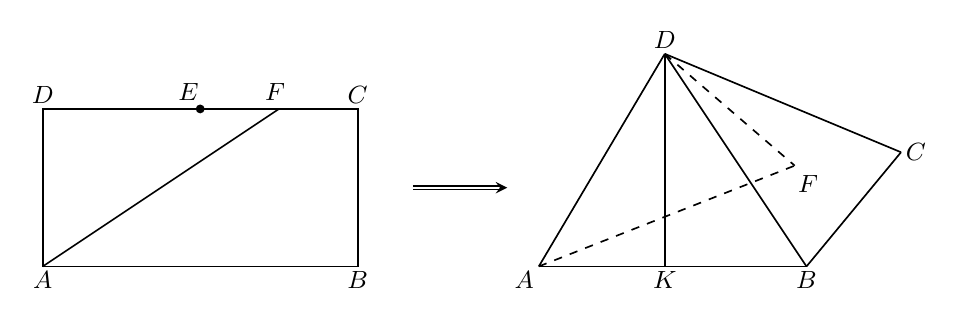
\begin{tikzpicture}[semithick, every node/.style={inner sep=1.5pt, font=\small}]

  % ---------- 折前 ----------
  \draw (0,0) rectangle (4,2);
  \draw (0,0) -- (3,2);
  \fill (2,2) circle (1.6pt);
  \node[above] at (0,2) {$D$};
  \node[above] at (1.85,2.05) {$E$};
  \node[above] at (2.95,2.05) {$F$};
  \node[above] at (4,2) {$C$};
  \node[below] at (0,0) {$A$};
  \node[below] at (4,0) {$B$};

  % ---------- 箭头 ----------
  \draw[double, ->, >=stealth] (4.7,1.0) -- (5.9,1.0) node[midway, above] {};

  % ---------- 折后 ----------
  \coordinate (A) at (6.3,0);
  \coordinate (K) at (7.9,0);
  \coordinate (B) at (9.7,0);
  \coordinate (D) at (7.9,2.7);
  \coordinate (C) at (10.9,1.45);
  \coordinate (F) at (9.55,1.28);
  \draw (A) -- (B);
  \draw (A) -- (D);
  \draw (D) -- (K);
  \draw (D) -- (B);
  \draw (B) -- (C);
  \draw (D) -- (C);
  \draw[dashed] (A) -- (F);
  \draw[dashed] (D) -- (F);
  \node[below left] at (A) {$A$};
  \node[below] at (K) {$K$};
  \node[below] at (B) {$B$};
  \node[above] at (D) {$D$};
  \node[right] at (C) {$C$};
  \node[below] at (9.72,1.22) {$F$};
\end{tikzpicture}
\end{center}
\nopagebreak[4]
\Needspace{4\baselineskip}
\textbf{解析}

在长方形所在平面内取 $A(0,0)$，$B(2,0)$，$C(2,1)$，$D(0,1)$，则 $E(1,1)$，$F(s,1)$，其中 $F$ 在线段 $EC$ 内部，故 $1<s<2$。

折起后记 $D$ 的位置为 $D'$。平面 $ABD'$ 与平面 $ABC$（即 $z=0$）垂直，且二者交于 $AB$（$x$ 轴），故 $D'$ 在过 $AB$ 的竖直平面内，设 $D'(t,0,h)$。$K$ 是 $D'$ 在 $AB$ 上的垂足，故 $K(t,0,0)$，$AK=t$。

\Needspace{5\baselineskip}
折叠不改变 $A$ 到 $D$、$F$ 到 $D$ 的距离：

\nopagebreak[4]
\[t^2+h^2=|AD'|^2=|AD|^2=1,\]

\nopagebreak[4]
\[(s-t)^2+(0-1)^2+h^2=|D'F|^2=|DF|^2=s^2.\]

第二式减去第一式得 $(s-t)^2+1-t^2=s^2-1$，即 $s^2-2st+1=s^2-1$，故 $st=1$，$t=\dfrac1s$。

$1<s<2$ 时 $t=\dfrac1s$ 取遍 $\left(\dfrac12,1\right)$，且 $h=\sqrt{1-t^2}>0$ 恒有意义（$t<1$）。故 $t$ 的取值范围是 $\left(\dfrac12,1\right)$。

端点说明：$s=1$（$F$ 与 $E$ 重合）时 $t=1$，$s=2$（$F$ 与 $C$ 重合）时 $t=\dfrac12$，题设“端点除外”故两端不取。

\gkanswer{答案：$\left(\dfrac12,1\right)$。}

\end{answer}
\begin{answer}
\gksolhead{18}{}

\textbf{题目}：

在 $\triangle ABC$ 中，角 $A$，$B$，$C$ 所对的边分别为 $a$，$b$，$c$，且满足 $\cos\dfrac A2=\dfrac{2\sqrt5}{5}$，$\overrightarrow{AB}\cdot\overrightarrow{AC}=3$．

（1）求 $\triangle ABC$ 的面积；

（2）若 $b+c=6$，求 $a$ 的值．

\Needspace{4\baselineskip}
\textbf{解析}

（1）由 $\cos\dfrac A2=\dfrac{2\sqrt5}{5}$ 得 $\cos A=2\cos^2\dfrac A2-1=2\times\dfrac45-1=\dfrac35$，故 $\sin A=\dfrac45$（$A$ 为三角形内角）。

$\overrightarrow{AB}\cdot\overrightarrow{AC}=|\overrightarrow{AB}||\overrightarrow{AC}|\cos A=bc\cdot\dfrac35=3$，得 $bc=5$。

面积 $S=\dfrac12bc\sin A=\dfrac12\times5\times\dfrac45=2$。

\Needspace{5\baselineskip}
（2）由余弦定理

\nopagebreak[4]
\[a^2=b^2+c^2-2bc\cos A=(b+c)^2-2bc-2bc\cdot\frac35=36-10-6=20,\]

故 $a=2\sqrt5$。

检验：$bc=5$，$b+c=6$ 给出 $\{b,c\}=\{5,1\}$，此时 $a^2=25+1-2\times5\times\dfrac35=20$，与上式一致。

\gkanswer{答案：（1）$2$；（2）$a=2\sqrt5$。}

\end{answer}
\begin{answer}
\gksolhead{19}{}

\textbf{题目}：

在 $1$，$2$，$3$，$\cdots$，$9$ 这 $9$ 个自然数中，任取 $3$ 个数．

（1）求这 $3$ 个数中恰有 $1$ 个是偶数的概率；

（2）设 $\xi$ 为这 $3$ 个数中两数相邻的组数（例如：若取出的数为 $1$，$2$，$3$，则有两组相邻的数 $1$，$2$ 和 $2$，$3$，此时 $\xi$ 的值是 $2$）．求随机变量 $\xi$ 的分布列及其数学期望 $E\xi$．

\Needspace{4\baselineskip}
\textbf{解析}

（1）$1$—$9$ 中偶数 $2,4,6,8$ 共 $4$ 个，奇数共 $5$ 个。恰有 $1$ 个偶数的取法为 $\mathrm C_4^1\mathrm C_5^2=4\times10=40$，总取法 $\mathrm C_9^3=84$，概率为 $\dfrac{40}{84}=\dfrac{10}{21}$。

（2）$\xi$ 的取值只能是 $0$，$1$，$2$（三个数至多组成两组相邻数）。

\begin{itemize}
\item $\xi=2$：三数两两相邻，即三个连续整数 $\{k,k+1,k+2\}$，$k=1,\dots,7$，共 $7$ 组；
\item $\xi=0$：三数两两不相邻。把三数记为 $a<b<c$，令 $a'=a$，$b'=b-1$，$c'=c-2$，则 $a'<b'<c'$ 是 $1$—$7$ 中的三个不同数，反之亦然，故共 $\mathrm C_7^3=35$ 组；
\item $\xi=1$：$84-7-35=42$ 组。
\end{itemize}

\Needspace{5\baselineskip}
故分布列为

\nopagebreak[4]
\[P(\xi=0)=\frac{35}{84}=\frac{5}{12},\qquad P(\xi=1)=\frac{42}{84}=\frac12,\qquad P(\xi=2)=\frac{7}{84}=\frac1{12},\]

\Needspace{5\baselineskip}
数学期望

\nopagebreak[4]
\[E\xi=0\times\frac{5}{12}+1\times\frac12+2\times\frac1{12}=\frac{42+14}{84}=\frac23.\]

（另法：$8$ 个相邻数对中每一对同时被取到的概率为 $\dfrac{\mathrm C_7^1}{\mathrm C_9^3}=\dfrac{7}{84}$，故 $E\xi=8\times\dfrac{7}{84}=\dfrac23$，与分布列一致。）

\gkanswer{答案：（1）$\dfrac{10}{21}$；（2）$P(\xi=0)=\dfrac{5}{12}$，$P(\xi=1)=\dfrac12$，$P(\xi=2)=\dfrac1{12}$，$E\xi=\dfrac23$。}

\end{answer}
\begin{answer}
\gksolhead{20}{}

\textbf{题目}：

如图，平面 $PAC\perp$ 平面 $ABC$，$\triangle ABC$ 是以 $AC$ 为斜边的等腰直角三角形，$E$，$F$，$O$ 分别为 $PA$，$PB$，$AC$ 的中点，$AC=16$，$PA=PC=10$．

（1）设 $G$ 是 $OC$ 的中点，证明：$FG\parallel$ 平面 $BOE$；

（2）证明：在 $\triangle ABO$ 内存在一点 $M$，使 $FM\perp$ 平面 $BOE$，并求点 $M$ 到 $OA$，$OB$ 的距离．
\nopagebreak[4]
\begin{center}% 2009 年浙江卷理科第 20 题：四棱锥 P-ABC 型立体图（平面 PAC⊥平面 ABC）。
% 来源 PDF：普通高考/2009/2009浙江理.pdf，SHA-256 8b9a62d8af65c0049a04b2c462e5bc8dc66a464244ca2c2462c6cdfafc5c2d89。
% 原页：第 2 页第 1 栏中部，书页码 566。
% 重绘依据：A 在左、C 在右、B 在前下方，P 在 AC 中垂面上；E∈PA、F∈PB、
%   O 为 AC 中点、G 为 OC 中点。实线为可见棱 PA、PB、PC、AB、BC 与 BE；
%   虚线为 AC（过 O）、BO、EO、FG。
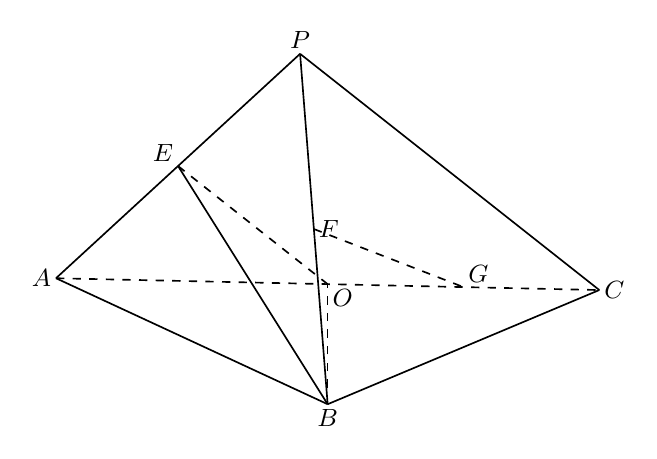
\begin{tikzpicture}[semithick, every node/.style={inner sep=1.5pt, font=\small}]
  \coordinate (P) at (3.1,4.6);
  \coordinate (A) at (0,1.75);
  \coordinate (C) at (6.9,1.60);
  \coordinate (O) at (3.45,1.675);
  \coordinate (B) at (3.45,0.15);
  \coordinate (E) at (1.55,3.175);
  \coordinate (F) at (3.275,2.375);
  \coordinate (G) at (5.175,1.6375);

  \draw (P) -- (A);
  \draw (P) -- (B);
  \draw (P) -- (C);
  \draw (A) -- (B);
  \draw (B) -- (C);
  \draw (E) -- (B);

  \draw[dashed] (A) -- (C);
  \draw[dashed] (B) -- (O);
  \draw[dashed] (E) -- (O);
  \draw[dashed] (F) -- (G);

  \node[above] at (P) {$P$};
  \node[left] at (A) {$A$};
  \node[below] at (B) {$B$};
  \node[right] at (C) {$C$};
  \node[above left] at (E) {$E$};
  \node[right] at (F) {$F$};
  \node[above right] at (G) {$G$};
  \node[below right] at (O) {$O$};
\end{tikzpicture}
\end{center}
\nopagebreak[4]
\Needspace{4\baselineskip}
\textbf{解析}

由 $AC=16$，$O$ 为 $AC$ 中点，得 $AO=OC=8$。$\triangle ABC$ 是以 $AC$ 为斜边的等腰直角三角形，故 $OB\perp AC$ 且 $OB=\dfrac{AC}{2}=8$。平面 $PAC\perp$ 平面 $ABC$，$PA=PC=10$，故 $P$ 在 $AC$ 的中垂面上，$PO\perp$ 平面 $ABC$，$PO=\sqrt{10^2-8^2}=6$。

取 $O$ 为原点，$OA$，$OB$，$OP$ 分别为 $x$，$y$，$z$ 轴，则

$A(-8,0,0)$，$C(8,0,0)$，$B(0,8,0)$，$P(0,0,6)$，

$E(-4,0,3)$，$F(0,4,3)$，$G(4,0,0)$。

\Needspace{5\baselineskip}
（1）$\overrightarrow{FG}=(4,-4,-3)$。平面 $BOE$ 过 $O$，由 $\overrightarrow{OB}=(0,8,0)$，$\overrightarrow{OE}=(-4,0,3)$ 得法向量

\nopagebreak[4]
\[\boldsymbol n=\overrightarrow{OB}\times\overrightarrow{OE}=(24,0,32).\]

$\overrightarrow{FG}\cdot\boldsymbol n=4\times24+0+(-3)\times32=96-96=0$，故 $FG$ 平行于平面 $BOE$；又 $\boldsymbol n\cdot\overrightarrow{OF}=0+0+96=96\neq0$，即 $F$ 不在平面 $BOE$ 内，所以 $FG\parallel$ 平面 $BOE$。

\Needspace{5\baselineskip}
（2）$\boldsymbol n=(24,0,32)\parallel(3,0,4)$。若 $FM\perp$ 平面 $BOE$，则 $M$ 在过 $F$ 且方向为 $(3,0,4)$ 的直线上，设

\nopagebreak[4]
\[M=(3\lambda,\,4,\,3+4\lambda).\]

\Needspace{5\baselineskip}
$M$ 在 $\triangle ABO$ 内，而 $\triangle ABO$ 位于平面 $z=0$，故 $3+4\lambda=0$，$\lambda=-\dfrac34$，得

\nopagebreak[4]
\[M\left(-\frac94,\,4,\,0\right).\]

检验 $M\in\triangle ABO$：$A(-8,0,0)$，$B(0,8,0)$，$O(0,0,0)$ 所围三角形为 $x\leqslant0$，$y\geqslant0$，$y\leqslant x+8$；$M$ 满足 $-2.25\leqslant0$，$4\geqslant0$，$4\leqslant5.75$，确在其内。

$M$ 到 $OA$（$x$ 轴）的距离为 $|y_M|=4$，到 $OB$（$y$ 轴）的距离为 $|x_M|=\dfrac94$。

\gkanswer{答案：（1）证明见解析；（2）$M$ 存在，$M$ 到 $OA$ 的距离为 $4$，到 $OB$ 的距离为 $\dfrac94$。}

\end{answer}
\begin{answer}
\gksolhead{21}{}

\textbf{题目}：

已知椭圆 $C_1:\dfrac{y^2}{a^2}+\dfrac{x^2}{b^2}=1$（$a>b>0$）的右顶点为 $A(1,0)$，过 $C_1$ 的焦点且垂直长轴的弦长为 $1$．

（1）求椭圆 $C_1$ 的方程；

（2）设点 $P$ 在抛物线 $C_2:y=x^2+h$（$h\in\mathbf R$）上，$C_2$ 在点 $P$ 处的切线与 $C_1$ 交于点 $M$，$N$．当线段 $AP$ 的中点与 $MN$ 的中点的横坐标相等时，求 $h$ 的最小值．

\Needspace{4\baselineskip}
\textbf{解析}

（1）椭圆 $\dfrac{y^2}{a^2}+\dfrac{x^2}{b^2}=1$（$a>b>0$）的长轴在 $y$ 轴上，$x$ 轴上的顶点为 $(\pm b,0)$。由右顶点 $A(1,0)$ 得 $b=1$。

焦点为 $(0,\pm c)$，$c^2=a^2-b^2$。过焦点且垂直于长轴（$y$ 轴）的弦是水平弦，其端点的横坐标满足 $\dfrac{c^2}{a^2}+\dfrac{x^2}{b^2}=1$，即 $x=\pm\dfrac{b^2}{a}$，弦长为 $\dfrac{2b^2}{a}$。由题设 $\dfrac{2}{a}=1$，得 $a=2$。

故 $C_1:\dfrac{y^2}{4}+x^2=1$（$c=\sqrt3$）。

\Needspace{5\baselineskip}
（2）设 $P(t,t^2+h)$，$C_2$ 在 $P$ 处的切线为

\nopagebreak[4]
\[y=2t(x-t)+t^2+h=2tx-t^2+h.\]

\Needspace{5\baselineskip}
代入 $C_1$：$\dfrac{(2tx-t^2+h)^2}{4}+x^2=1$，整理得

\nopagebreak[4]
\[(4t^2+4)x^2+4t(h-t^2)x+(h-t^2)^2-4=0.\]

\Needspace{5\baselineskip}
设交点横坐标为 $x_M$，$x_N$，则

\nopagebreak[4]
\[x_M+x_N=-\frac{4t(h-t^2)}{4t^2+4}=-\frac{t(h-t^2)}{1+t^2},\]

\Needspace{5\baselineskip}
$MN$ 中点的横坐标为 $-\dfrac{t(h-t^2)}{2(1+t^2)}$；$AP$ 中点的横坐标为 $\dfrac{1+t}{2}$。令二者相等：

\nopagebreak[4]
\[\frac{1+t}{2}=-\frac{t(h-t^2)}{2(1+t^2)}\ \Longrightarrow\ (1+t)(1+t^2)=-t(h-t^2)\ \Longrightarrow\ h=-1-t-\frac1t.\]

\Needspace{5\baselineskip}
判别式大于零等价于 $(h-t^2)^2<4(1+t^2)$。把 $h$ 代入并化简得

\nopagebreak[4]
\[(t+1)^2(t^2+1)<4t^2,\]

\Needspace{5\baselineskip}
即 $t^4+2t^3-2t^2+2t+1<0$，也即 $(t^2+(1+\sqrt5)t+1)(t^2+(1-\sqrt5)t+1)<0$。第二个因式恒正，故条件等价于

\nopagebreak[4]
\[\frac{-(1+\sqrt5)-\sqrt{2+2\sqrt5}}{2}<t<\frac{-(1+\sqrt5)+\sqrt{2+2\sqrt5}}{2},\]

即 $-2.890\cdots<t<-0.346\cdots$，

\Needspace{5\baselineskip}
特别地 $t<0$。记 $u=-t>0$，则

\nopagebreak[4]
\[h=-1+u+\frac1u\geqslant-1+2=1,\]

等号在 $u=1$（即 $t=-1$）时成立，此时 $h=1$，$h-t^2=0$，判别式为 $4(1+1)=8>0$，$M$，$N$ 确为不同两点（切线 $y=-2x$ 与椭圆交于 $\left(\pm\dfrac{\sqrt2}{2},\mp\sqrt2\right)$）。

故 $h$ 的最小值为 $1$。

\gkanswer{答案：（1）$\dfrac{y^2}{4}+x^2=1$；（2）$h$ 的最小值为 $1$。}

\end{answer}
\begin{answer}
\gksolhead{22}{}

\textbf{题目}：

已知函数 $f(x)=x^3-(k^2-k+1)x^2+5x-2$，$g(x)=k^2x^2+kx+1$，其中 $k\in\mathbf R$．

（1）设函数 $p(x)=f(x)+g(x)$．若 $p(x)$ 在区间 $(0,3)$ 上不单调，求 $k$ 的取值范围；

（2）设函数 $q(x)=\begin{cases}g(x),&x\geqslant0,\\f(x),&x<0.\end{cases}$ 是否存在 $k$，对任意给定的非零实数 $x_1$，存在唯一的非零实数 $x_2$（$x_2\neq x_1$），使得 $q'(x_2)=q'(x_1)$ 成立？若存在，求 $k$ 的值；若不存在，请说明理由．

\Needspace{4\baselineskip}
\textbf{解析}

\Needspace{5\baselineskip}
（1）$p(x)=f(x)+g(x)=x^3+(k-1)x^2+(k+5)x-1$，

\nopagebreak[4]
\[p'(x)=3x^2+2(k-1)x+(k+5).\]

\Needspace{5\baselineskip}
$p$ 在 $(0,3)$ 上不单调，等价于 $p'$ 在 $(0,3)$ 内有变号零点。计算三个关键值：

\nopagebreak[4]
\[p'(0)=k+5,\qquad p'(3)=27+6(k-1)+(k+5)=7k+26,\]

\Needspace{5\baselineskip}
顶点 $x_0=\dfrac{1-k}{3}$ 处

\nopagebreak[4]
\[p'(x_0)=-\frac{(k-1)^2}{3}+(k+5)=\frac{-k^2+5k+14}{3}=-\frac{(k-7)(k+2)}{3}.\]

情形一：$p'(0)p'(3)<0$，即 $(k+5)(7k+26)<0$，得 $-5<k<-\dfrac{26}{7}$。此时 $p'$ 在 $(0,3)$ 内恰有一个变号零点。

情形二：顶点在 $(0,3)$ 内（$-8<k<1$）且 $p'(x_0)<0$（$k<-2$ 或 $k>7$），此时 $p'$ 在 $(0,3)$ 内有两个零点，但还需 $p'(0)>0$ 且 $p'(3)>0$，即 $k>-\dfrac{26}{7}$，故得 $-\dfrac{26}{7}<k<-2$。

合并得 $-5<k<-2$。其余情形单调：$k=-5$ 时 $p'=3x^2-12x=3x(x-4)$，在 $(0,3)$ 上恒负；$k=-2$ 时 $p'=3(x-1)^2\geqslant0$；$-8<k<-5$ 时 $p'(0)<0$，$p'(3)<0$，顶点又在 $(0,3)$ 内，故 $p'<0$ 恒成立；$k\leqslant-8$ 或 $k\geqslant1$ 时 $p'$ 在 $(0,3)$ 内不变号。

（2）$x>0$ 时 $q'(x)=2k^2x+k$；$x<0$ 时 $q'(x)=3x^2-2(k^2-k+1)x+5$。

注意 $k^2-k+1=\left(k-\dfrac12\right)^2+\dfrac34>0$，故 $x<0$ 时 $q'(x)$ 的对称轴 $x=\dfrac{k^2-k+1}{3}>0$，它在 $(-\infty,0)$ 上严格递减，值域为 $(5,+\infty)$（$x\to0^-$ 时趋于 $5$，$x\to-\infty$ 时趋于 $+\infty$）。

$x>0$ 时若 $k\neq0$，$q'(x)$ 严格递增，值域为 $(k,+\infty)$；若 $k=0$，$q'\equiv0$，对 $x_1>0$ 有无穷多个 $x_2$，不合要求。以下设 $k\neq0$。

对 $x_1>0$：$v=q'(x_1)=2k^2x_1+k$ 取遍 $(k,+\infty)$。$x>0$ 一侧只有 $x_1$ 使 $q'=v$，故 $x<0$ 一侧必须恰有一个解，即要求 $v>5$ 对一切 $v\in(k,+\infty)$ 成立，得 $k\geqslant5$。

对 $x_1<0$：$v=q'(x_1)>5$。$x<0$ 一侧只有 $x_1$ 使 $q'=v$，故 $x>0$ 一侧必须恰有一个解，即 $x_2=\dfrac{v-k}{2k^2}>0$，要求 $v>k$ 对一切 $v>5$ 成立，得 $k\leqslant5$。

两条件同时成立当且仅当 $k=5$。当 $k=5$ 时，两支的值域都是 $(5,+\infty)$ 且各自严格单调，任一非零 $x_1$ 在另一侧恰有唯一的 $x_2$ 与之对应，且 $x_2$ 与 $x_1$ 异号故 $x_2\neq x_1$，$x_2\neq0$ 也成立。故存在，$k=5$。

检验 $k=5$：$x>0$ 时 $q'=50x+5$，值域 $(5,+\infty)$；$x<0$ 时 $q'=3x^2-42x+5$，值域 $(5,+\infty)$ 且严格递减。对 $x_1=1$，$v=55$，对侧解 $3x^2-42x+5=55$ 即 $x^2-14x-50/3=0$，负根 $x_2=7-\sqrt{197/3}\approx-1.10\neq1$，唯一。

\gkanswer{答案：（1）$-5<k<-2$；（2）存在，$k=5$。}

\end{answer}